% !TEX program = xelatex
\documentclass{resume} % 简历文档类（自带图标、datedsubsection等基础命令）

% 1. 仅保留必要宏包（删除冲突项，避免重复加载）
\usepackage{graphicx}               % 图片插入（必选）
\usepackage{zh_CN-Adobefonts_external} % 中文Adobe字体（必选，确保中文显示）
\usepackage{url}                    % URL格式支持（必选）
\usepackage{geometry}               % 页边距调整（必选）
\usepackage{xcolor}                 % 颜色定义（仅加载1次，解决darkgreen未定义）
\usepackage{hyperref}               % 链接功能（最后加载，避免冲突）

% 2. 页边距配置（适配文本宽度，减少Overfull）
\geometry{top=0.8cm, bottom=1.5cm, left=1.4cm, right=1.4cm} % 左右边距各减0.1cm，避免超宽

% 3. 颜色与链接配置（保持原风格，兼容打印）
\definecolor{darkgreen}{RGB}{0, 100, 0} % 定义深绿色
\hypersetup{
	colorlinks=true,
	linkcolor=blue,
	urlcolor=darkgreen,
	breaklinks=true,
	unicode=true,
	pdfstartview=FitH
}

% 4. 重新定义“稍粗+深色”样式（颜色调深，粗细可按需调整）
% 颜色：gray!50（比原来的gray!70深很多）
% 粗细：\bfseries（粗体）+ 11pt字号（比原来的10.5pt稍大，更突出）
\newcommand{\highlight}[1]{{\bfseries\fontsize{13pt}{13pt}\selectfont\textcolor{gray!90}{#1}}}

\begin{document}
	\pagenumbering{gobble} % 隐藏页码
	
	% 个人信息区（保持原布局，无修改）
	\vspace*{-10pt}
	\noindent
	\begin{tabular}{@{}p{0.64\textwidth}@{\hspace{0.02\textwidth}}p{0.34\textwidth}@{}}
		\centering
		\LARGE\bfseries 张建\\[6pt]
		\normalsize
		求职意向：AI产品经理/Agent开发工程师\\[3pt]
		个人网站：\href{https://husterzj.info/}{\textcolor{black}{HUSTERZJ.INFO}}\\[3pt]
		\faEnvelope\ m202473806@hust.edu.cn\\[3pt]
		\faPhone\ 15237776378 \hspace{1em} \faCalendar\ 25岁
		&
		\raggedleft
		\vspace{-30pt}
		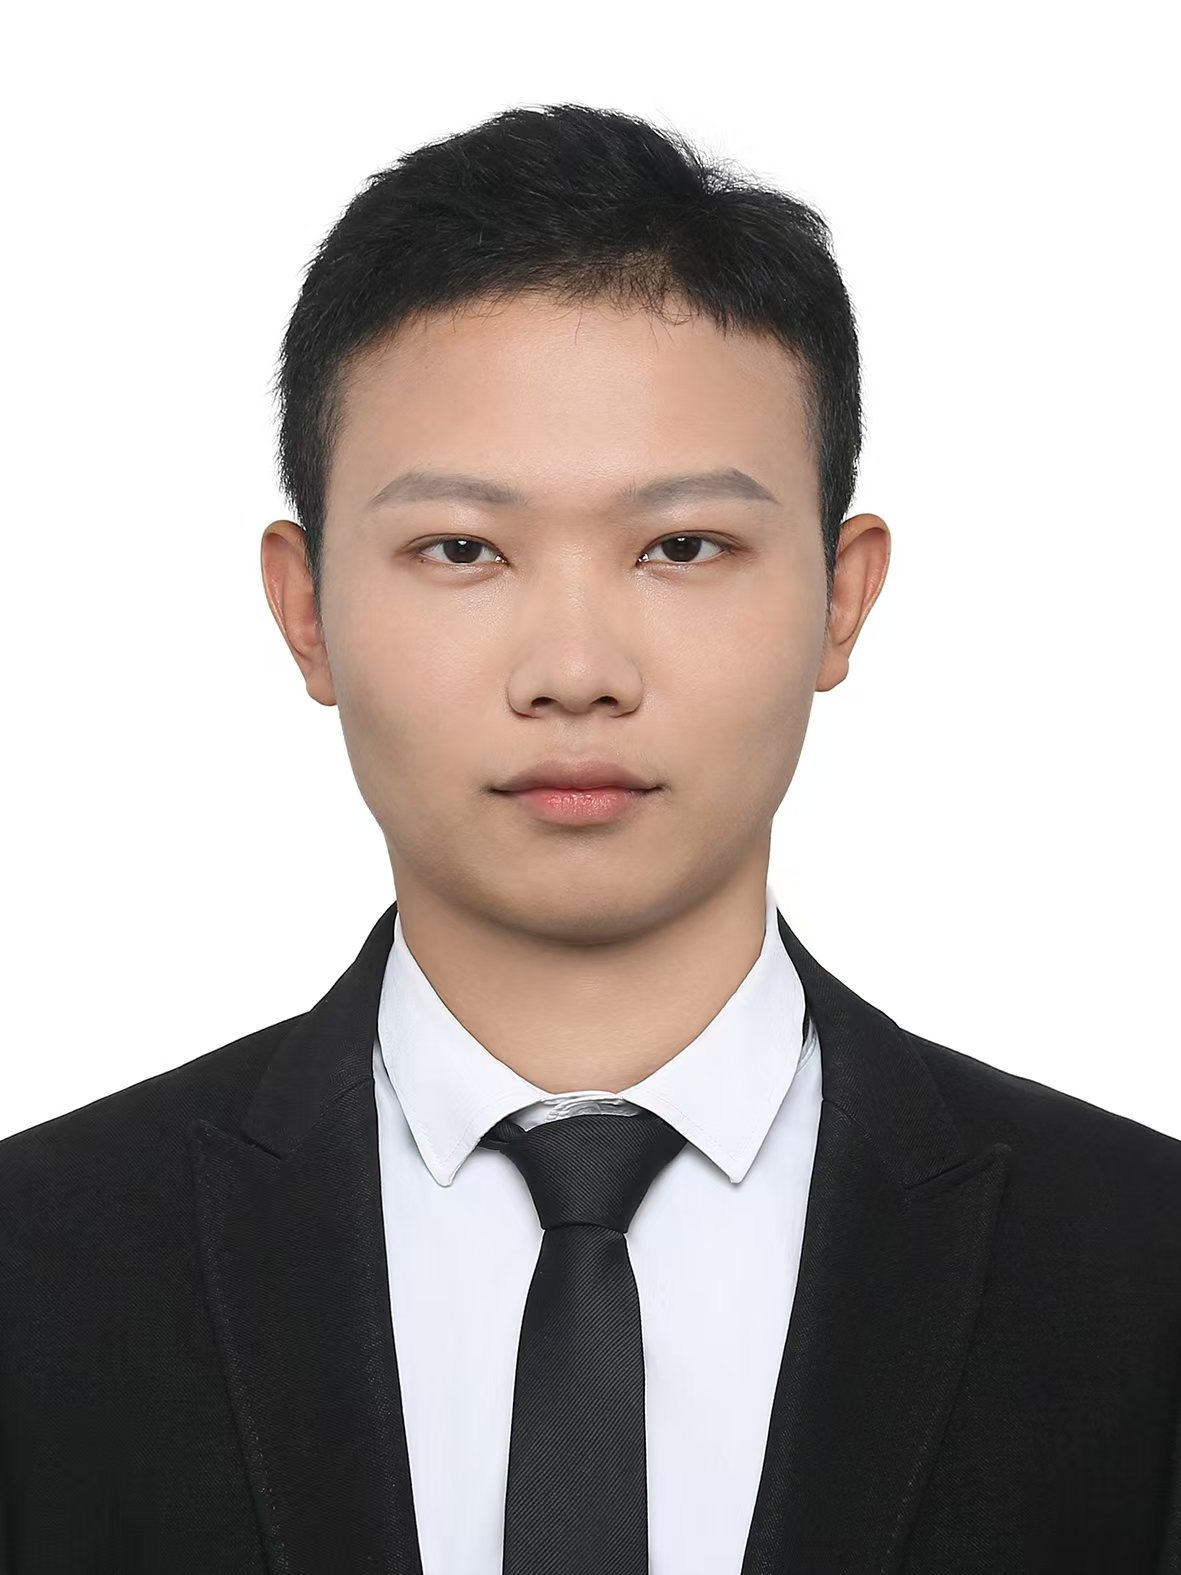
\includegraphics[width=1.05in]{zj} % 确保图片文件“zj”在当前目录（如zj.jpg/png）
	\end{tabular}
	\vspace{-5pt}
	
	\section{\faCog\ 专业技能}
	\begin{itemize}[parsep=0.5ex] % 紧凑列表，避免冗余
		\item AI技术与应用：熟悉大模型微调、Agent SKills、Harness Engineering等技术以及Openclaw等Agent框架，能结合业务场景设计落地方案
		\item 需求分析与产品工具应用：具备从0到1需求分析、业务流程拆解能力；熟练使用产品原型工具（Figma/Axure/墨刀），能独立完成需求梳理、原型设计、项目文档沉淀
		\item 项目管理与协作：具备跨角色协作能力；可通过会议主持、目标拆解、分工协调推动项目落地
		\item 技术与开发基础：熟练掌握ClaudeCode / Cursor等AIcoding工具使用技巧；精通Git；较熟悉Python、JavaScript编程；了解Vue前端及FastAPI/Django框架
	\end{itemize}
	
	\section{\faGraduationCap\ 教育经历}
	\datedsubsection{\textbf{华中科技大学} \hspace{1em} \textit{人工智能与自动化学院 - 智能科学与技术学硕}}{2024.9 -- 至今}
	主修课程：智能计算系统、机器人导论、现代最优化理论与方法等
	
	\datedsubsection{\textbf{华中科技大学} \hspace{1em} \textit{人工智能与自动化学院 - 自动化专业工学学士}}{2019.9 -- 2024.6}
	专业排名前5\%。主修课程：模式识别、计算机网络、数据结构、C语言、数据库等
	
	\section{\faBriefcase\ 项目经历}
	% 减小hspace间距（从3em→2em），解决Overfull \hbox

	\datedsubsection{\textbf{航天器任务调度原型系统开发} \hspace{1em} \textit{国自然重点项目 \hspace{2em} \href{https://astroscheduler.cn/}{https://astroscheduler.cn/}}}{2024.5 -- 至今}
	\large {简要介绍：研发通用调度分析工具软件，为复杂航天任务提供全流程支持}
	\begin{itemize}
		\item 目标：让用户可以在几分钟内定义复杂的航天器任务调度问题，选择合适的算法并配置参数得到解决方案，并通过甘特图或表格图形化显示
		\item 模块划分：规划包、资源和任务管理、约束定义、算法配置、调度结果分析六大核心模块
		\item 主要贡献：主导软件系统开发全流程，包括需求分析、界面设计、数据库设计、接口设计、原型系统开发等
	\end{itemize}
	
	\datedsubsection{\textbf{基于模型的Aicoding科研方向探索} \hspace{2em} \textit{科研项目} }{2025.4 -- 至今}
	\large {简要介绍：探索 AI Coding 新范式，推动研发流程从“基于对话(Chat)”和“基于文档(Document)”向“基于模型(Model)”的架构演进。}
	\begin{itemize}
		\item mbse理论深度实践：深度参与杭州华望系统工程专项研修，系统掌握MBSE核心理论；能够熟练运用MagicDraw等建模工具进行系统级需求、行为及结构建模，具备将复杂业务逻辑转化为规范化模型的能力。
		\item 高水平论文发表：撰写学术论文《基于MBSE的航天任务调度工具系统模型构建》，目前已投递至航天领域顶级期刊《载人航天》；文中详细阐述了如何通过模型驱动提升航天调度系统的逻辑一致性与研制效率。
		\item 核心技术专利申请：作为主要发明人申请专利 《一种模型驱动的软件开发全流程自动生成方法及系统》；该专利提出了一种利用模型语义直接生成代码的创新架构。
	\end{itemize}
	
	\datedsubsection{\textbf{华中科技大学 MBA《AI 赋能管理创新》课程代课讲师} \hspace{2em} \textit{教育培训} }{2025.4 -- 至今}
	\large {项目概述：受邀担任管理学院 MBA 班级实操课主讲，旨在提升高级管理人才的 AI 战略视野与工具链应用能力。}
	\begin{itemize}
		\item AI 核心技术内化：系统讲解提示词工程、RAG、模型微调及 智能体工作流等前沿概念，帮助学生构建从基础原理到业务场景适配的认知闭环。
		\item 前沿开发工具实操：指导学生完成 Cursor、Claude Code 等AI原生编程工具的部署与实战，演示如何利用AI提升业务流程自动化水平
		\item 智能体框架落地指导：深度解析OpenClaw智能体框架，带教环境搭建、Skill开发及多Agent协作技巧，培养学生设计可落地的企业级 AI Agent 方案能力。
	\end{itemize}
	
	\datedsubsection{\textbf{开源项目汇总研究导航} \hspace{1em} \textit{个人项目 \hspace{2em}  \href{https://roadmap.sh/r/rdm-ud9x6}{https://roadmap.sh/r/rdm-ud9x6}}}{2022.9 -- 至今}
	\large {简要介绍：为满足个人学习复盘、对外交流分享需求，结合 ROADMAP 开源工具与飞书，系统汇总分类整理了值得深入学习与借鉴的开源项目，形成结构化导航体系。}
	\begin{itemize}
		\item 软件类：按应用场景划分，涵盖LLM、软件开发、教程、工具等，覆盖技术学习与实践全场景
		\item 硬件类：围绕硬件开发全流程分类，包含硬件项目案例、硬件设计与调试工具、教程等
		\item 项目分类：为项目按照关注程度打标签，划分为尝试复现、稍微感兴趣、非常感兴趣等
		\item 深入理解：针对重点项目撰写核心介绍并附加飞书文档链接及外部优质资源链接
	\end{itemize}	
	
	\section{\faUser\ 自我评价}
	形成一套自己为人处世的第一性原理并长期坚持，信奉长期主义，热爱看论文以及听深度访谈博客，有非常强的创新性思维，梦想是做一款伟大的产品
	
	\section{\faFileImageO\ 附件 - 相关页面}
	\begin{center}
		% 第一张图：航天器任务调度原型系统
		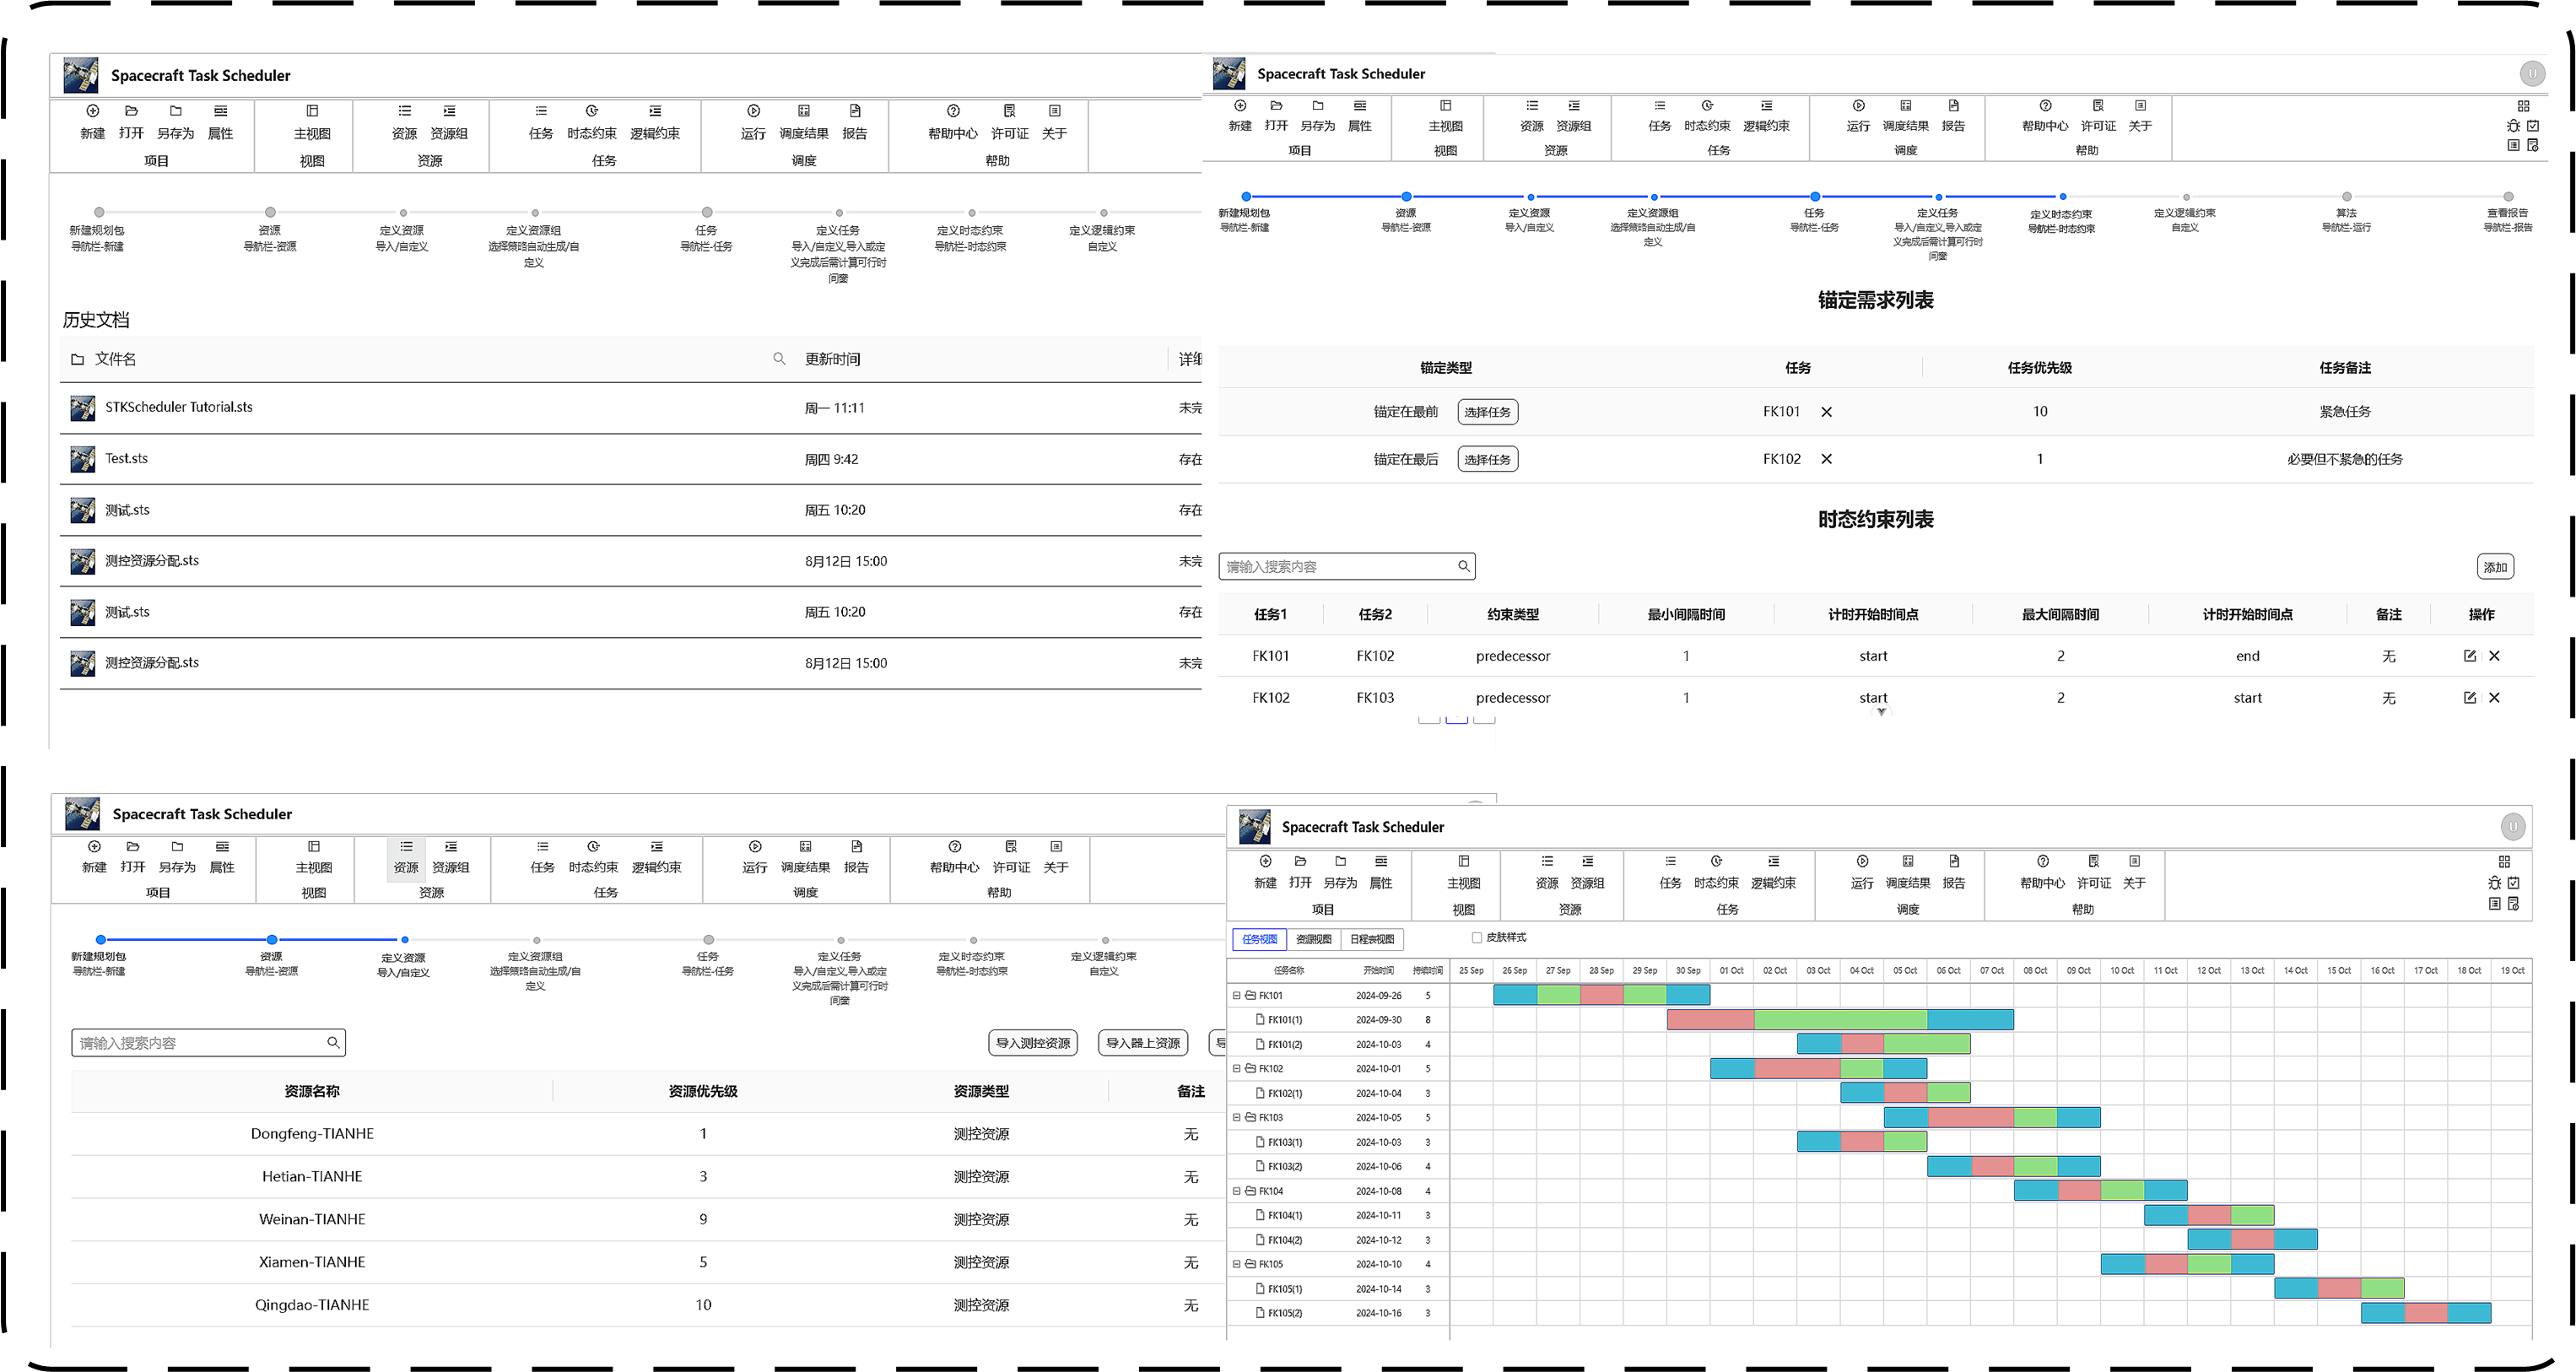
\includegraphics[width=1\textwidth]{fujian/7_航天器任务调度原型系统.png} \\[5pt]
		\small\centering 航天器任务调度原型系统 \\[15pt] % 图下方说明文字，加15pt间距分隔两张图
		
	\end{center}
	
\end{document}